\makeatletter
\def\input@path{{./}{../}{../../}{../../../}{../../../../}{preamble/}{../preamble/}{../../preamble/}{../../../preamble/}}
\makeatother
\input{preamble.tex}

\geometry{
	top=0.5cm,
	bottom=0.5cm,
	left=0.5cm,
	right=0.5cm
}


\usepackage{booktabs}
\usepackage{tikz}
\usepackage{pgfplots}

\pgfplotsset{compat=1.18}
\usetikzlibrary{patterns}
\usetikzlibrary{arrows.meta}
\usetikzlibrary{calc}
\usetikzlibrary{intersections}
\usepgfplotslibrary{fillbetween}



\pagestyle{empty}
\setlength{\parindent}{0pt}
\renewcommand{\arraystretch}{1.02}

\begin{document}
	
	% ==========================================================
	% STANDARD NORMAL DISTRIBUTION
	% ==========================================================
	
	\begin{center}
		{\Large\textbf{Standard Normal Distribution Reference Sheet}}
	\end{center}
	
	\vspace{-7mm}
	
	\noindent
	\begin{minipage}[t]{0.68\textwidth}
		\vspace{0pt}
		
		\textbf{How to read the table.}
		
		Let
		\[
		Z\sim\mathcal{N}(0,1)
		\qquad \textrm{with} \qquad
		\Phi(z)=P(Z\le z)
		\]
		The table gives the area to the left of a positive \(z\)-value under the
		standard normal curve. The left column gives the ones and tenths digits
		of \(z\), while the top row gives the hundredths digit.
		
		\vspace{2mm}
		\begin{center}
			\fbox{%
				\begin{minipage}{0.72\textwidth}
					\textbf{Example}: For
					\vspace{-6mm}
					\[
					\qquad \quad \Phi(1.23)=P(Z\le1.23)=0.8907
					\]
					
					\vspace{-4mm}
					
					look for row \(1.2\) and column \(0.03\).
					
					\vspace{2mm}
				\end{minipage}%
			}
		\end{center}
	\end{minipage}%
	\hfill
	\begin{minipage}[t]{0.28\textwidth}
		\vspace{0pt}
		\centering 
		
		\textbf{Useful identities} \vspace{-8mm}
		
		\begin{gather*}
			P(Z>z)=1-\Phi(z),\\
			\Phi(-z)=1-\Phi(z),\\
			P(a<Z<b)=\Phi(b)-\Phi(a),\\
			P(|Z|>a)=2[1-\Phi(a)].
		\end{gather*}
		\[
		\begin{aligned}
			\Phi &:\ \textrm{Phi} \\
			\phi &:\ \textrm{phi}
		\end{aligned}
		\]
	\end{minipage}
	
	\begin{center}
		\begin{minipage}{0.55\textwidth}
			\begin{center}
				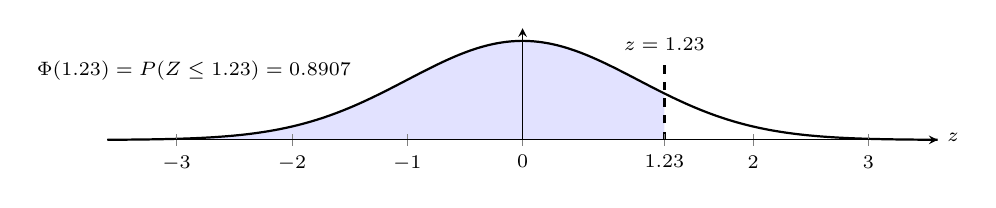
\begin{tikzpicture}
					\begin{axis}[
						width=\linewidth,
						height=3.0cm,
						axis lines=middle,
						axis on top,
						set layers=standard,
						xmin=-3.6,
						xmax=3.6,
						ymin=0,
						ymax=0.45,
						samples=180,
						domain=-3.6:3.6,
						xtick={-3,-2,-1,2,3},
						extra x ticks={0,1.23},
						extra x tick labels={$0$,$1.23$},
						extra x tick style={
							tick label style={
								font=\scriptsize,
								yshift=-2pt,
								fill=white,
								inner sep=1pt
							}
						},
						ytick=\empty,
						xlabel={\(z\)},
						xlabel style={
							font=\scriptsize,
							at={(axis description cs:1,0.02)},
							anchor=west
						},
						tick label style={font=\scriptsize},
						clip=false
						]
						
						\addplot[
						draw=none,
						fill=blue!25,
						fill opacity=0.45,
						domain=-3.6:1.23,
						samples=120,
						on layer=axis background
						]
						{1/sqrt(2*pi)*exp(-x^2/2)}
						\closedcycle;
						
						\addplot[
						thick,
						black,
						domain=-3.6:3.6
						]
						{1/sqrt(2*pi)*exp(-x^2/2)};
						
						\draw[dashed, line width=1.2pt]
						(axis cs:1.23,0) -- (axis cs:1.23,0.32);
						
						\node[
						anchor=south,
						font=\scriptsize
						] at (axis cs:1.23,0.32)
						{\(z=1.23\)};
						
						\node[
						anchor=center,
						align=center,
						font=\scriptsize
						] at (axis cs:-2.85,0.28)
						{\(\Phi(1.23)=P(Z\le1.23)=0.8907\)};
						
					\end{axis}
				\end{tikzpicture}
			\end{center}
		\end{minipage}
		\begin{minipage}{0.25\textwidth}
			\centering 
			Probability density function 
			\vspace*{-3mm}
			\[
			\boxed{f_Z(z)=
			\frac{1}{\sqrt{2\pi}}
			e^{-z^2/2}
			}
			\]
		\end{minipage}
	\end{center}
	
	\begin{center}
		\noindent\textbf{Standard normal table: values of \(\Phi(z)=P(Z\le z)\)}
	\end{center}
	
	\begin{center}
		\renewcommand{\arraystretch}{1}
		\setlength{\tabcolsep}{10.2pt}
		\arrayrulecolor{gray!95}
		\rowcolors{2}{gray!33}{white}
		
		\begin{tabular}{|c!{\color{black!85}\vrule width 1.8pt}c|c|c|c|c|c|c|c|c|c|}
			\hline
			\rowcolor{gray!60}
			\(z\) & 0.00 & 0.01 & 0.02 & 0.03 & 0.04 & 0.05 & 0.06 & 0.07 & 0.08 & 0.09\\
			\hline
			0.0 & 0.5000 & 0.5040 & 0.5080 & 0.5120 & 0.5160 & 0.5199 & 0.5239 & 0.5279 & 0.5319 & 0.5359\\
			0.1 & 0.5398 & 0.5438 & 0.5478 & 0.5517 & 0.5557 & 0.5596 & 0.5636 & 0.5675 & 0.5714 & 0.5753\\
			0.2 & 0.5793 & 0.5832 & 0.5871 & 0.5910 & 0.5948 & 0.5987 & 0.6026 & 0.6064 & 0.6103 & 0.6141\\
			0.3 & 0.6179 & 0.6217 & 0.6255 & 0.6293 & 0.6331 & 0.6368 & 0.6406 & 0.6443 & 0.6480 & 0.6517\\
			0.4 & 0.6554 & 0.6591 & 0.6628 & 0.6664 & 0.6700 & 0.6736 & 0.6772 & 0.6808 & 0.6844 & 0.6879\\
			0.5 & 0.6915 & 0.6950 & 0.6985 & 0.7019 & 0.7054 & 0.7088 & 0.7123 & 0.7157 & 0.7190 & 0.7224\\
			0.6 & 0.7257 & 0.7291 & 0.7324 & 0.7357 & 0.7389 & 0.7422 & 0.7454 & 0.7486 & 0.7517 & 0.7549\\
			0.7 & 0.7580 & 0.7611 & 0.7642 & 0.7673 & 0.7704 & 0.7734 & 0.7764 & 0.7794 & 0.7823 & 0.7852\\
			0.8 & 0.7881 & 0.7910 & 0.7939 & 0.7967 & 0.7995 & 0.8023 & 0.8051 & 0.8078 & 0.8106 & 0.8133\\
			0.9 & 0.8159 & 0.8186 & 0.8212 & 0.8238 & 0.8264 & 0.8289 & 0.8315 & 0.8340 & 0.8365 & 0.8389\\
			1.0 & 0.8413 & 0.8438 & 0.8461 & 0.8485 & 0.8508 & 0.8531 & 0.8554 & 0.8577 & 0.8599 & 0.8621\\
			1.1 & 0.8643 & 0.8665 & 0.8686 & 0.8708 & 0.8729 & 0.8749 & 0.8770 & 0.8790 & 0.8810 & 0.8830\\
			1.2 & 0.8849 & 0.8869 & 0.8888 & 0.8907 & 0.8925 & 0.8944 & 0.8962 & 0.8980 & 0.8997 & 0.9015\\
			1.3 & 0.9032 & 0.9049 & 0.9066 & 0.9082 & 0.9099 & 0.9115 & 0.9131 & 0.9147 & 0.9162 & 0.9177\\
			1.4 & 0.9192 & 0.9207 & 0.9222 & 0.9236 & 0.9251 & 0.9265 & 0.9279 & 0.9292 & 0.9306 & 0.9319\\
			1.5 & 0.9332 & 0.9345 & 0.9357 & 0.9370 & 0.9382 & 0.9394 & 0.9406 & 0.9418 & 0.9429 & 0.9441\\
			1.6 & 0.9452 & 0.9463 & 0.9474 & 0.9484 & 0.9495 & 0.9505 & 0.9515 & 0.9525 & 0.9535 & 0.9545\\
			1.7 & 0.9554 & 0.9564 & 0.9573 & 0.9582 & 0.9591 & 0.9599 & 0.9608 & 0.9616 & 0.9625 & 0.9633\\
			1.8 & 0.9641 & 0.9649 & 0.9656 & 0.9664 & 0.9671 & 0.9678 & 0.9686 & 0.9693 & 0.9699 & 0.9706\\
			1.9 & 0.9713 & 0.9719 & 0.9726 & 0.9732 & 0.9738 & 0.9744 & 0.9750 & 0.9756 & 0.9761 & 0.9767\\
			2.0 & 0.9772 & 0.9778 & 0.9783 & 0.9788 & 0.9793 & 0.9798 & 0.9803 & 0.9808 & 0.9812 & 0.9817\\
			2.1 & 0.9821 & 0.9826 & 0.9830 & 0.9834 & 0.9838 & 0.9842 & 0.9846 & 0.9850 & 0.9854 & 0.9857\\
			2.2 & 0.9861 & 0.9864 & 0.9868 & 0.9871 & 0.9875 & 0.9878 & 0.9881 & 0.9884 & 0.9887 & 0.9890\\
			2.3 & 0.9893 & 0.9896 & 0.9898 & 0.9901 & 0.9904 & 0.9906 & 0.9909 & 0.9911 & 0.9913 & 0.9916\\
			2.4 & 0.9918 & 0.9920 & 0.9922 & 0.9925 & 0.9927 & 0.9929 & 0.9931 & 0.9932 & 0.9934 & 0.9936\\
			2.5 & 0.9938 & 0.9940 & 0.9941 & 0.9943 & 0.9945 & 0.9946 & 0.9948 & 0.9949 & 0.9951 & 0.9952\\
			\hline
		\end{tabular}
		
		\arrayrulecolor{black}
	\end{center}
	
	
	\newpage
	
% ==========================================================
% STUDENT'S T-DISTRIBUTION
% ==========================================================

\begin{center}
	{\Large\textbf{Student's \(t\)-Distribution Reference Sheet}}
\end{center}

\vspace{0.1cm}

\noindent
\begin{minipage}[t]{0.68\textwidth}
	\vspace{0pt}
	
	\textbf{How to read the table.}
	
	Let
	\vspace{-3mm}
	\[
	T\sim t_{\nu},
	\qquad
	\textrm{where } \nu \textrm{ is the number of degrees of freedom (df)}
	\]
	
	For a sample of size \(n\), we have that
	$
	\nu=n-1.
	$
	The table gives positive critical values \(t^*_{\alpha,\nu}\), defined by
	\[
	P\!\left(T>t^*_{\alpha,\nu}\right)=\alpha
	\]
	
	The left column gives the degrees of freedom \(\nu\). Select the column
	corresponding to the desired tail probability \(\alpha\).
	
	\vspace{2mm}
	
\end{minipage}%
\hfill
\begin{minipage}[t]{0.28\textwidth}
	\vspace{0pt}
	\centering
	\textbf{Useful identities}
	\vspace{-2mm}
	\begin{gather*}
		P\!\left(T>t^*_{\alpha,\nu}\right)=\alpha,\\
		P\!\left(T<-t^*_{\alpha,\nu}\right)=\alpha,\\
		P\!\left(|T|>t^*_{\alpha,\nu}\right)=2\alpha,\\
		P\!\left(-t^*_{\alpha,\nu}<T<t^*_{\alpha,\nu}\right)=1-2\alpha.
	\end{gather*}
	\[
	\begin{aligned}
		\alpha &:\ \textrm{alpha} \\
		\nu    &:\ \textrm{nu}
	\end{aligned}
	\]
	
\end{minipage}

\begin{center}
	\fbox{%
		\begin{minipage}{0.72\textwidth}
			\textbf{Example}: For \(\nu=10\) and \(\alpha=0.025\),
			\vspace{-6mm}
			\[
			\qquad \quad t^*=2.228
			\]
			
			\vspace{-1mm}
			
			so
			\vspace{-6mm}
			\[
			P(T>2.228)=P(T<-2.228)=0.025
			\]
			
			
			and therefore
			\vspace{-6mm}
			\[
			P(-2.228<T<2.228)=1-2(0.025)=0.95.
			\]
			
		\end{minipage}%
	}
\end{center}

\begin{center}
	\begin{minipage}{0.55\textwidth}
		\begin{center}
			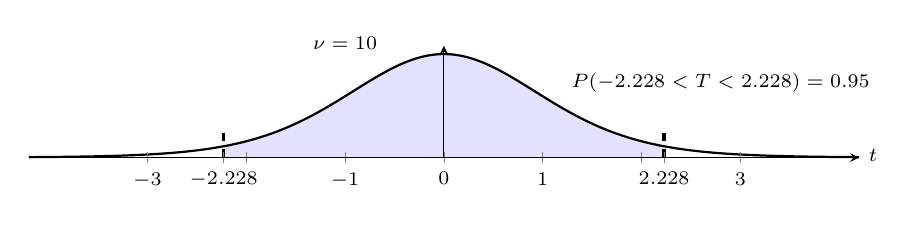
\begin{tikzpicture}
				\begin{axis}[
					width=\linewidth,
					height=3.0cm,
					axis lines=middle,
					axis on top,
					set layers=standard,
					xmin=-4.2,
					xmax=4.2,
					ymin=0,
					ymax=0.42,
					samples=180,
					domain=-4.2:4.2,
					xtick={-3,-2,-1,1,2,3},
					extra x ticks={0,-2.228,2.228},
					extra x tick labels={$0$,$-2.228$,$2.228$},
					extra x tick style={
						tick label style={
							font=\scriptsize,
							yshift=-2pt,
							fill=white,
							inner sep=1pt
						}
					},
					ytick=\empty,
					xlabel={\(t\)},
					xlabel style={
						font=\scriptsize,
						at={(axis description cs:1,0.02)},
						anchor=west
					},
					tick label style={font=\scriptsize},
					clip=false
					]
					
					% Central 95% area for nu = 10
					\addplot[
					draw=none,
					fill=blue!25,
					fill opacity=0.45,
					domain=-2.228:2.228,
					samples=120,
					on layer=axis background
					]
					{
						0.389108383966
						*(1+x^2/10)^(-5.5)
					}
					\closedcycle;
					
					% Student's t density for nu = 10
					\addplot[
					thick,
					black,
					domain=-4.2:4.2
					]
					{
						0.389108383966
						*(1+x^2/10)^(-5.5)
					};
					
					\draw[dashed, line width=1.2pt]
					(axis cs:-2.228,0) -- (axis cs:-2.228,0.12);
					
					\draw[dashed, line width=1.2pt]
					(axis cs:2.228,0) -- (axis cs:2.228,0.12);
					
					\node[
					anchor=center,
					align=center,
					font=\scriptsize
					] at (axis cs:2.8,0.28)
					{\(P(-2.228<T<2.228)=0.95\)};
					
					\node[
					anchor=south,
					font=\scriptsize
					] at (axis cs:-1,0.37)
					{\(\nu=10\)};
					
				\end{axis}
			\end{tikzpicture}
		\end{center}
	\end{minipage}
	\begin{minipage}{0.37\textwidth}
		\centering
		Probability density function \vspace*{-3mm}
		\[
		\boxed{f_T(t)=
		\frac{
			\Gamma\!\left(\frac{\nu+1}{2}\right)
		}{
			\sqrt{\nu\pi}\,
			\Gamma\!\left(\frac{\nu}{2}\right)
		}
		\left(
		1+\frac{t^2}{\nu}
		\right)^{-\frac{\nu+1}{2}}
		}
		\]
	\end{minipage}
\end{center}

\begin{center}
	\noindent\textbf{Student's \(t\) critical values \(t^*\)}
\end{center}

\begin{center}
	\renewcommand{\arraystretch}{1}
	\setlength{\tabcolsep}{4.4pt}
	\arrayrulecolor{gray!95}
	
	\begin{minipage}[t]{0.49\textwidth}
		\centering
		\rowcolors{3}{gray!33}{white}
		
		\begin{tabular}{
				|c
				!{\color{black!85}\vrule width 1.8pt}
				c|c|c|c|c|c|
			}
			\hline
			
			\rowcolor{gray!60}
			\(\nu\)
			&
			\multicolumn{6}{c|}{\textbf{Tail probability \(\alpha\)}}\\
			
			\cline{2-7}
			
			\rowcolor{gray!60}
			\textbf{df}
			& 0.20
			& 0.10
			& 0.05
			& 0.025
			& 0.01
			& 0.005\\
			
			\hline
			
			1  & 1.376 & 3.078 & 6.314 & 12.706 & 31.821 & 63.657\\
			2  & 1.061 & 1.886 & 2.920 & 4.303  & 6.965  & 9.925\\
			3  & 0.978 & 1.638 & 2.353 & 3.182  & 4.541  & 5.841\\
			4  & 0.941 & 1.533 & 2.132 & 2.776  & 3.747  & 4.604\\
			5  & 0.920 & 1.476 & 2.015 & 2.571  & 3.365  & 4.032\\
			6  & 0.906 & 1.440 & 1.943 & 2.447  & 3.143  & 3.707\\
			7  & 0.896 & 1.415 & 1.895 & 2.365  & 2.998  & 3.499\\
			8  & 0.889 & 1.397 & 1.860 & 2.306  & 2.896  & 3.355\\
			9  & 0.883 & 1.383 & 1.833 & 2.262  & 2.821  & 3.250\\
			10 & 0.879 & 1.372 & 1.812 & 2.228  & 2.764  & 3.169\\
			11 & 0.876 & 1.363 & 1.796 & 2.201  & 2.718  & 3.106\\
			12 & 0.873 & 1.356 & 1.782 & 2.179  & 2.681  & 3.055\\
			13 & 0.870 & 1.350 & 1.771 & 2.160  & 2.650  & 3.012\\
			14 & 0.868 & 1.345 & 1.761 & 2.145  & 2.624  & 2.977\\
			15 & 0.866 & 1.341 & 1.753 & 2.131  & 2.602  & 2.947\\
			16 & 0.865 & 1.337 & 1.746 & 2.120  & 2.583  & 2.921\\
			17 & 0.863 & 1.333 & 1.740 & 2.110  & 2.567  & 2.898\\
			18 & 0.862 & 1.330 & 1.734 & 2.101  & 2.552  & 2.878\\
			19 & 0.861 & 1.328 & 1.729 & 2.093  & 2.539  & 2.861\\
			20 & 0.860 & 1.325 & 1.725 & 2.086  & 2.528  & 2.845\\
			
			\hline
		\end{tabular}
	\end{minipage}
	\hfill
	\begin{minipage}[t]{0.49\textwidth}
		\centering
		\rowcolors{3}{gray!33}{white}
		
		\begin{tabular}{
				|c
				!{\color{black!85}\vrule width 1.8pt}
				c|c|c|c|c|c|
			}
			\hline
			
			\rowcolor{gray!60}
			\(\nu\)
			&
			\multicolumn{6}{c|}{\textbf{Tail probability \(\alpha\)}}\\
			
			\cline{2-7}
			
			\rowcolor{gray!60}
			\textbf{df}
			& 0.20
			& 0.10
			& 0.05
			& 0.025
			& 0.01
			& 0.005\\
			
			\hline
			
			21  & 0.859 & 1.323 & 1.721 & 2.080 & 2.518 & 2.831\\
			22  & 0.858 & 1.321 & 1.717 & 2.074 & 2.508 & 2.819\\
			23  & 0.858 & 1.319 & 1.714 & 2.069 & 2.500 & 2.807\\
			24  & 0.857 & 1.318 & 1.711 & 2.064 & 2.492 & 2.797\\
			25  & 0.856 & 1.316 & 1.708 & 2.060 & 2.485 & 2.787\\
			26  & 0.856 & 1.315 & 1.706 & 2.056 & 2.479 & 2.779\\
			27  & 0.855 & 1.314 & 1.703 & 2.052 & 2.473 & 2.771\\
			28  & 0.855 & 1.313 & 1.701 & 2.048 & 2.467 & 2.763\\
			29  & 0.854 & 1.311 & 1.699 & 2.045 & 2.462 & 2.756\\
			30  & 0.854 & 1.310 & 1.697 & 2.042 & 2.457 & 2.750\\
			35  & 0.852 & 1.306 & 1.690 & 2.030 & 2.438 & 2.724\\
			40  & 0.851 & 1.303 & 1.684 & 2.021 & 2.423 & 2.704\\
			45  & 0.850 & 1.301 & 1.679 & 2.014 & 2.412 & 2.690\\
			50  & 0.849 & 1.299 & 1.676 & 2.009 & 2.403 & 2.678\\
			60  & 0.848 & 1.296 & 1.671 & 2.000 & 2.390 & 2.660\\
			80  & 0.846 & 1.292 & 1.664 & 1.990 & 2.374 & 2.639\\
			100 & 0.845 & 1.290 & 1.660 & 1.984 & 2.364 & 2.626\\
			120 & 0.845 & 1.289 & 1.658 & 1.980 & 2.358 & 2.617\\
			200 & 0.843 & 1.286 & 1.653 & 1.972 & 2.345 & 2.601\\
			
			\hline
			
			\(\infty\)
			& 0.842
			& 1.282
			& 1.645
			& 1.960
			& 2.326
			& 2.576\\
			
			\hline
		\end{tabular}
	\end{minipage}
	
	\arrayrulecolor{black}
\end{center}


\end{document}